%&../../.preamble
\endofdump

\usetikzlibrary{external}
\tikzset{external/system call={pdflatex --shell-escape --fmt=../../.preamble --halt-on-error -jobname "\image" "\endofdump\texsource"}}
\tikzexternalize[prefix=tikz/]

\title{Esame 07/2025}

\begin{document}
\maketitle
\section{Esercizio 1}
Calcolare tabella e indicare i conflitti di shift/reduce e reduce/reduce. Dire se viene parsata la stringa \verb|acb|
\vskip3mm

% Grammar
\begin{align*}
	S & \rightarrow aSb \mid cA \mid Bc \mid AB \\
	A & \rightarrow aSb \mid cA                 \\
	B & \rightarrow Bc \mid \epsilon            \\
\end{align*}

\vskip3mm
\sfblue{Soluzione:} \href{https://mdaines.github.io/grammophone/?s=UyAtPiBhIFM
	gYiB8IGMgQSB8IEIgYyB8IEEgQiAuCkEgLT4gYSBTIGIgfCBjIEEgLgpCI
	C0+IEIgYyB8ICAuCg==}{grammatica su Grammophone}
%
,
\href{https://dreampuf.github.io/GraphvizOnline/?engine=do
t#digraph%20G%20%7B%0Anode%5Bshape%3Drecord%5D%0A%0A0%20%5
Blabel%3D%22%7B%200%20%7C%20%40%20%E2%86%92%20%E2%80%A2S%5
Cn%20%7C%20S%20%E2%86%92%20%E2%80%A2aSb%5CnS%20%E2%86%92%2
0%E2%80%A2cA%5CnS%20%E2%86%92%20%E2%80%A2Bc%5CnS%20%E2%86%
92%20%E2%80%A2AB%5CnA%20%E2%86%92%20%E2%80%A2aSb%5CnA%20%E
2%86%92%20%E2%80%A2cA%5CnB%20%E2%86%92%20%E2%80%A2Bc%5CnB%
20%E2%86%92%20%E2%80%A2%5Cn%20%7D%22%5D%0A1%20%5Blabel%3D%
22%7B%201%20%7C%20%40%20%E2%86%92%20S%E2%80%A2%5Cn%20%7D%2
2%5D%0A2%20%5Blabel%3D%22%7B%202%20%7C%20S%20%E2%86%92%20a
%E2%80%A2Sb%5CnA%20%E2%86%92%20a%E2%80%A2Sb%5Cn%20%7C%20S%
20%E2%86%92%20%E2%80%A2aSb%5CnS%20%E2%86%92%20%E2%80%A2cA%
5CnS%20%E2%86%92%20%E2%80%A2Bc%5CnS%20%E2%86%92%20%E2%80%A
2AB%5CnA%20%E2%86%92%20%E2%80%A2aSb%5CnA%20%E2%86%92%20%E2
%80%A2cA%5CnB%20%E2%86%92%20%E2%80%A2Bc%5CnB%20%E2%86%92%2
0%E2%80%A2%5Cn%20%7D%22%5D%0A3%20%5Blabel%3D%22%7B%203%20%
7C%20S%20%E2%86%92%20c%E2%80%A2A%5CnA%20%E2%86%92%20c%E2%8
0%A2A%5Cn%20%7C%20A%20%E2%86%92%20%E2%80%A2aSb%5CnA%20%E2%
86%92%20%E2%80%A2cA%5Cn%20%7D%22%5D%0A4%20%5Blabel%3D%22%7
B%204%20%7C%20S%20%E2%86%92%20A%E2%80%A2B%5Cn%20%7C%20B%20
%E2%86%92%20%E2%80%A2Bc%5CnB%20%E2%86%92%20%E2%80%A2%5Cn%2
0%7D%22%5D%0A5%20%5Blabel%3D%22%7B%205%20%7C%20S%20%E2%86%
92%20B%E2%80%A2c%5CnB%20%E2%86%92%20B%E2%80%A2c%5Cn%20%7D%
22%5D%0A6%20%5Blabel%3D%22%7B%206%20%7C%20S%20%E2%86%92%20
aS%E2%80%A2b%5CnA%20%E2%86%92%20aS%E2%80%A2b%5Cn%20%7D%22%
5D%0A7%20%5Blabel%3D%22%7B%207%20%7C%20S%20%E2%86%92%20cA%
E2%80%A2%5CnA%20%E2%86%92%20cA%E2%80%A2%5Cn%20%7D%22%5D%0A
8%20%5Blabel%3D%22%7B%208%20%7C%20A%20%E2%86%92%20a%E2%80%
A2Sb%5Cn%20%7C%20S%20%E2%86%92%20%E2%80%A2aSb%5CnS%20%E2%8
6%92%20%E2%80%A2cA%5CnS%20%E2%86%92%20%E2%80%A2Bc%5CnS%20%
E2%86%92%20%E2%80%A2AB%5CnA%20%E2%86%92%20%E2%80%A2aSb%5Cn
A%20%E2%86%92%20%E2%80%A2cA%5CnB%20%E2%86%92%20%E2%80%A2Bc
%5CnB%20%E2%86%92%20%E2%80%A2%5Cn%20%7D%22%5D%0A9%20%5Blab
el%3D%22%7B%209%20%7C%20A%20%E2%86%92%20c%E2%80%A2A%5Cn%20
%7C%20A%20%E2%86%92%20%E2%80%A2aSb%5CnA%20%E2%86%92%20%E2%
80%A2cA%5Cn%20%7D%22%5D%0A10%20%5Blabel%3D%22%7B%2010%20%7
C%20S%20%E2%86%92%20AB%E2%80%A2%5CnB%20%E2%86%92%20B%E2%80
%A2c%5Cn%20%7D%22%5D%0A11%20%5Blabel%3D%22%7B%2011%20%7C%2
0S%20%E2%86%92%20Bc%E2%80%A2%5CnB%20%E2%86%92%20Bc%E2%80%A
2%5Cn%20%7D%22%5D%0A12%20%5Blabel%3D%22%7B%2012%20%7C%20S%
20%E2%86%92%20aSb%E2%80%A2%5CnA%20%E2%86%92%20aSb%E2%80%A2
%5Cn%20%7D%22%5D%0A13%20%5Blabel%3D%22%7B%2013%20%7C%20A%2
0%E2%86%92%20aS%E2%80%A2b%5Cn%20%7D%22%5D%0A14%20%5Blabel%
3D%22%7B%2014%20%7C%20A%20%E2%86%92%20cA%E2%80%A2%5Cn%20%7
D%22%5D%0A15%20%5Blabel%3D%22%7B%2015%20%7C%20B%20%E2%86%9
2%20Bc%E2%80%A2%5Cn%20%7D%22%5D%0A16%20%5Blabel%3D%22%7B%2
016%20%7C%20A%20%E2%86%92%20aSb%E2%80%A2%5Cn%20%7D%22%5D%0
A%0A%0A%2F%2Fnodes%0A13%20-%3E%2016%20%5Blabel%3D%22b%22%5
D%0A9%20-%3E%2014%20%5Blabel%3D%22A%22%5D%0A9%20-%3E%208%2
0%5Blabel%3D%22a%22%5D%0A9%20-%3E%209%20%5Blabel%3D%22c%22
%5D%0A4%20-%3E%2010%20%5Blabel%3D%22B%22%5D%0A8%20-%3E%201
3%20%5Blabel%3D%22S%22%5D%0A8%20-%3E%202%20%5Blabel%3D%22a
%22%5D%0A8%20-%3E%203%20%5Blabel%3D%22c%22%5D%0A8%20-%3E%2
04%20%5Blabel%3D%22A%22%5D%0A8%20-%3E%205%20%5Blabel%3D%22
B%22%5D%0A10%20-%3E%2015%20%5Blabel%3D%22c%22%5D%0A0%20-%3
E%201%20%5Blabel%3D%22S%22%5D%0A0%20-%3E%202%20%5Blabel%3D
%22a%22%5D%0A0%20-%3E%203%20%5Blabel%3D%22c%22%5D%0A0%20-%
3E%204%20%5Blabel%3D%22A%22%5D%0A0%20-%3E%205%20%5Blabel%3
D%22B%22%5D%0A5%20-%3E%2011%20%5Blabel%3D%22c%22%5D%0A6%20
-%3E%2012%20%5Blabel%3D%22b%22%5D%0A2%20-%3E%206%20%5Blabe
l%3D%22S%22%5D%0A2%20-%3E%202%20%5Blabel%3D%22a%22%5D%0A2%
20-%3E%203%20%5Blabel%3D%22c%22%5D%0A2%20-%3E%204%20%5Blab
el%3D%22A%22%5D%0A2%20-%3E%205%20%5Blabel%3D%22B%22%5D%0A3
%20-%3E%207%20%5Blabel%3D%22A%22%5D%0A3%20-%3E%208%20%5Bla
bel%3D%22a%22%5D%0A3%20-%3E%209%20%5Blabel%3D%22c%22%5D%0A
%7D%0A}{automa su Graphviz} 




% Lr0 parsing table
\begin{table}[H]\centering\ifcsname parsingTablesFontSize\endcsname \parsingTablesFontSize \fi
	\begin{tabular}{ccccccccc}
		\toprule
		States & a     & b     & c      & \$    & S  & A  & B  & Symbol map \\
		\midrule
		s0     & s2/r8 & r8    & s3/r8  & r8    & 1  & 4  & 5  & []         \\
		s1     &       &       &        & acc   &    &    &    & [S]        \\
		s2     & s2/r8 & r8    & s3/r8  & r8    & 6  & 4  & 5  & [a]        \\
		s3     & s8    &       & s9     &       &    & 7  &    & [c]        \\
		s4     & r8    & r8    & r8     & r8    &    &    & 10 & [A]        \\
		s5     &       &       & s11    &       &    &    &    & [B]        \\
		s6     &       & s12   &        &       &    &    &    & [aS]       \\
		s7     & r2/r6 & r2/r6 & r2/r6  & r2/r6 &    &    &    & [cA]       \\
		s8     & s2/r8 & r8    & s3/r8  & r8    & 13 & 4  & 5  & [ca]       \\
		s9     & s8    &       & s9     &       &    & 14 &    & [cc]       \\
		s10    & r4    & r4    & s15/r4 & r4    &    &    &    & [AB]       \\
		s11    & r3/r7 & r3/r7 & r3/r7  & r3/r7 &    &    &    & [Bc]       \\
		s12    & r1/r5 & r1/r5 & r1/r5  & r1/r5 &    &    &    & [aSb]      \\
		s13    &       & s16   &        &       &    &    &    & [caS]      \\
		s14    & r6    & r6    & r6     & r6    &    &    &    & [ccA]      \\
		s15    & r7    & r7    & r7     & r7    &    &    &    & [ABc]      \\
		s16    & r5    & r5    & r5     & r5    &    &    &    & [caSb]     \\
		\bottomrule
	\end{tabular}
	\caption{Tabella di parsing LR(0)}\end{table}


% Slr1 parsing table
\begin{table}[H]
	\centering
	\begin{tabular}{ccccccccc}
		\toprule
		States & a  & b     & c     & \$    & S  & A  & B  & Symbol map \\
		\midrule
		s0     & s2 & r8    & s3/r8 & r8    & 1  & 4  & 5  & []         \\
		s1     &    &       &       & acc   &    &    &    & [S]        \\
		s2     & s2 & r8    & s3/r8 & r8    & 6  & 4  & 5  & [a]        \\
		s3     & s8 &       & s9    &       &    & 7  &    & [c]        \\
		s4     &    & r8    & r8    & r8    &    &    & 10 & [A]        \\
		s5     &    &       & s11   &       &    &    &    & [B]        \\
		s6     &    & s12   &       &       &    &    &    & [aS]       \\
		s7     &    & r2/r6 & r6    & r2/r6 &    &    &    & [cA]       \\
		s8     & s2 & r8    & s3/r8 & r8    & 13 & 4  & 5  & [ca]       \\
		s9     & s8 &       & s9    &       &    & 14 &    & [cc]       \\
		s10    &    & r4    & s15   & r4    &    &    &    & [AB]       \\
		s11    &    & r3/r7 & r7    & r3/r7 &    &    &    & [Bc]       \\
		s12    &    & r1/r5 & r5    & r1/r5 &    &    &    & [aSb]      \\
		s13    &    & s16   &       &       &    &    &    & [caS]      \\
		s14    &    & r6    & r6    & r6    &    &    &    & [ccA]      \\
		s15    &    & r7    & r7    & r7    &    &    &    & [ABc]      \\
		s16    &    & r5    & r5    & r5    &    &    &    & [caSb]     \\
		\bottomrule
	\end{tabular}
	\caption{Tabella di parsing SLR(1)}\end{table}


% First-follow set
\begin{table}[H]\centering
	\begin{tabular}{cccc}
		\toprule
		Symbol & First\-set & Follow\-set & Nullable \\
		\midrule
		S      & a,c        & b,\$        & No       \\
		A      & a,c        & b,c,\$      & No       \\
		B      & c          & b,c,\$      & Yes      \\
		\bottomrule
	\end{tabular}
\end{table}
\section{Esercizio 2}
Scrivere tabella di parsing LL1 della seguente grammatica:
\begin{align*}
	S & \rightarrow  aSbA \mid bAaS \mid \epsilon \\
	A & \rightarrow  Aab \mid ba                  \\
\end{align*}

\vskip3mm
\sfblue{Soluzione:} \href{https://mdaines.github.io/grammophone/?s=UyAtPiBhIFMgYiBBIHwgYiBBIGEgUyB8IC4KQSAtPiBBIGEgYnwgYiBhIC4K}{Grammatica su Grammophone}

\begin{table}[h]
	\centering
	\begin{tabular}{c c c c }
		\toprule
		 & a                                                             & b & \$ \\
		\midrule
		S
		 & \(S \rightarrow a S b A\)
		 & \begin{tabular}[t]{@{}l@{}} % Conflict cell
			   \(S \rightarrow b A a S\) \\
			   \(S \rightarrow \epsilon\)
		   \end{tabular}
		 & \(S \rightarrow \epsilon\)                                             \\
		A
		 &
		 & \begin{tabular}[t]{@{}l@{}} % Conflict cell
			   \(A \rightarrow A a b\) \\
			   \(A \rightarrow b a\)
		   \end{tabular}
		 &                                                                        \\
		\bottomrule
	\end{tabular}
	\caption{Tabella di parsing LL(1)}
\end{table}


\section{Esercizio 3}
Dato
\begin{align*}
	r_1 & = \epsilon \mid b \mid \left(\epsilon  \mid b\right) \left(a \mid \epsilon \mid b\right)^{*} \left(a \mid \epsilon \mid b\right) \\
	r_2 & = b^{*}a \mid b^{*}a\left(\epsilon \mid a \mid b\right)^{*}
\end{align*}
trovare un DFA minimo per $ \mathcal{L}\left(r_1 r_2\right) $

\vskip3mm
\sfblue{Soluzione:}
\begin{center}
	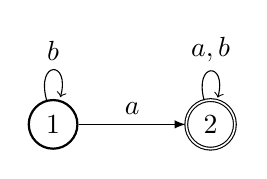
\begin{tikzpicture}
		\node (1)[draw, thick, circle] at (0,0) {1};
		\node (2)[draw, circle, double] at (2,0) {2};
		\draw [-latex](1)--(2) node [midway, above]{$ a $};
		\draw [-latex](1)edge[loop above] node [midway, above]{$ b $} (1);
		\draw [-latex](2)edge[loop above] node [midway, above]{$ a,b $} (2);
	\end{tikzpicture}
\end{center}

\section{Esercizio 4}
Dato $ r_1 = a^{*}b^{*}a^{*} $, trovare il DFA minimo per il linguaggio
\[
	\mathcal{L}\left(\left(a \mid b\right)^{*}\right) \setminus \mathcal{L}\left(r_1\right)
\]
\vskip3mm
\sfblue{Soluzione:}

\begin{center}
	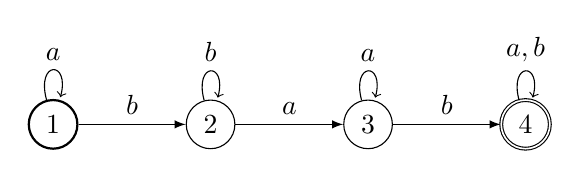
\begin{tikzpicture}
		\node (1)[draw, thick, circle] at (0,0) {1};
		\node (2)[draw, circle] at (2,0) {2};
		\node (3)[draw, circle] at (4,0) {3};
		\node (4)[draw, circle, double] at (6,0) {4};
		\draw [-latex](1)--(2) node [midway, above]{$ b $};
		\draw [-latex](2)--(3) node [midway, above]{$ a $};
		\draw [-latex](3)--(4) node [midway, above]{$ b $};

		\draw [-latex](1)edge[loop above] node [midway, above]{$ a $} (1);
		\draw [-latex](2)edge[loop above] node [midway, above]{$ b $} (2);
		\draw [-latex](3)edge[loop above] node [midway, above]{$ a $} (3);
		\draw [-latex](4)edge[loop above] node [midway, above]{$ a,b $} (4);
	\end{tikzpicture}
\end{center}
\section{Esercizio 5}
Scrivere il codice intermedio generato per il seguente codice:
\begin{center}
	\verb|if (a = b) while(true) a = a * b * c|
\end{center}

\vskip3mm
\sfblue{Soluzione:}
\begin{lstlisting}[language=, frame = none]
        IF a = b then GOTO L1
        GOTO L0
L1, L2:  
        GOTO L3
        L3: 
        T1 = a * b
        T2 = T1 * c
        a = T2
        GOTO L2
    L0:
\end{lstlisting}



\end{document}
